\documentclass[12pt,a4paper]{article}
\usepackage[legalpaper,margin=2cm]{geometry}
\usepackage[export]{adjustbox}
\usepackage{amsmath}
\usepackage{fancyhdr}
\usepackage{hyperref}
\usepackage{listings}
\usepackage{xcolor}
\usepackage{setspace}
\usepackage{enumitem}
\usepackage{lmodern}
\newcommand{\subscript}[2]{$#1_#2$}
\DeclareMathOperator*{\argmax}{arg\,max}

\onehalfspacing
\addtolength\jot{8pt}

\graphicspath{ {docs/} }

\hypersetup{
	colorlinks=true,
	pdfpagemode=FullScreen,
	pdftitle={Homework IV - Group 67}
}

\lstdefinestyle{Python}{
	basicstyle=\footnotesize\ttfamily,
	frame=single,
	keywordstyle=\color{red},
	numbers=left,
	numbersep=5pt,
	numberstyle=\tiny\color{gray},
	showspaces=false,
	showstringspaces=false,
	stringstyle=\color{blue},
	tabsize=4
}

\lstset{style=Python}

\pagestyle{fancy}
\fancyhf{}
\rhead{Group \textbf{67}}
\lhead{Aprendizagem 2022/23 - Homework IV}
\cfoot{Luís Câmara (99099) and Pedro Lobo (99115)}

\renewcommand{\thesection}{\Roman{section}}
\renewcommand{\thesubsection}{\arabic{subsection}}

\newcommand{\xone} {
	\begin{bmatrix}
		1 \\ 2
	\end{bmatrix}
}
\newcommand{\xtwo} {
	\begin{bmatrix}
		-1 \\ 1
	\end{bmatrix}
}
\newcommand{\xthree} {
	\begin{bmatrix}
		1 \\ 0
	\end{bmatrix}
}

\newcommand{\muone} {
	\begin{bmatrix}
		2 \\ 2
	\end{bmatrix}
}
\newcommand{\mutwo} {
	\begin{bmatrix}
		0 \\ 0
	\end{bmatrix}
}

\newcommand{\sigmaone} {
	\begin{bmatrix}
		2 & 1 \\
		1 & 2
	\end{bmatrix}
}
\newcommand{\sigmatwo} {
	\begin{bmatrix}
		2 & 0 \\
		0 & 2
	\end{bmatrix}
}

\newcommand{\detsigmaone} {
	\begin{vmatrix}
		2 & 1 \\
		1 & 2
	\end{vmatrix}
}
\newcommand{\detsigmatwo} {
	\begin{vmatrix}
		2 & 0 \\
		0 & 2
	\end{vmatrix}
}

\newcommand{\pione} {0.5}
\newcommand{\pitwo} {0.5}

% #1 - n
% #2 - k
% #3 - D
% #4 - \Sigma_k
% #5 - vmatrix \Sigma_k
% #6 - x
% #7 - \mu_k
% #8 - result
\newcommand{\xmidc}[8] {
	\begin{flalign*}
		                                                                                                         & P(x_#1 \mid c_#2) = \mathcal{N}(x_#1 \mid \mu_#2, \Sigma_#2) = & \\
		                                                                                                         & = \frac{1}{(2\pi)^\frac{#3}{2} \cdot {#5}^\frac{1}{2}} \cdot
		e^{-\frac{1}{2} \left({#6} - {#7}\right)^\top \cdot \left(#4\right)^{-1} \cdot \left({#6} - {#7}\right)} &                                                                  \\
		                                                                                                         & = #8
	\end{flalign*}
}

% #1 - n
% #2 - k
% #3 - N result
% #4 - pi_k result
% #5 - result
\newcommand{\xc}[5] {
	\begin{flalign*}
		 & P(x_#1, c_#2) = \mathcal{N}(x_#1 \mid \mu_#2, \Sigma_#2) \cdot \pi_#2 = {#3} \times {#4} = #5 &
	\end{flalign*}
}

% #1 - n
% #2 - v1
% #3 - v2
% #4 - result
\newcommand{\x}[4] {
	\begin{flalign*}
		 & P(x_#1) = \sum_{k=1}^3 (\pi_k \cdot \mathcal{N}(x_#1 \mid \mu_k, \Sigma_k)) = {#2} + {#3} = #4 &
	\end{flalign*}
}

% #1 - n
% #2 - k
% #3 - v1
% #4 - v2
% #5 - result
\newcommand{\gam}[5] {
	\begin{flalign*}
		 & \gamma_{#2#1} = \frac{P(x_#1, c_#2)}{P(x_#1)} = \frac{#3}{#4} = #5 &
	\end{flalign*}
}

% #1 - k
% #2 - v1
% #3 - v2
% #4 - v3
% #5 - result
\newcommand{\n}[5] {
	\begin{flalign*}
		N_#1 & = \sum_{n=1}^3 \gamma_{#1n} = {#2} + {#3} + {#4} = #5 &
	\end{flalign*}
}

% #1 - k
% #2 - N
% #3 - v1
% #4 - x1
% #5 - v2
% #6 - x2
% #7 - v3
% #8 - x3
% #9 - result
\newcommand{\muupdate}[9] {
	\begin{flalign*}
		\mu_#1 & = \frac{1}{N_#1} \cdot \sum_{n=1}^3 \gamma_{#1n} \cdot x_n                              & \\
		       & = \frac{1}{#2} \cdot \left( {#3} \cdot {#4} + {#5} \cdot {#6} + {#7} \cdot {#8} \right) & \\
		       & = #9
	\end{flalign*}
}

% #1 - k
% #2 - N
% #3 - u_k
% #4 - gamma_kn
% #5 - gamma_kn
% #6 - gamma_kn
% #7 - result
\newcommand{\sigmaupdate}[7] {
	\begin{flalign*}
		\Sigma_#1 & = \frac{1}{N_#1} \cdot \sum_{n=1}^{3} \gamma_{#1n} \cdot (x_n - \mu_#1) \cdot (x_n - \mu_#1)^\top                   & \\
		          & = \frac{1}{#2} \cdot \left( {#4} \cdot \left( \xone - {#3} \right) \cdot \left( \xone - {#3} \right)^\top \right.   & \\
		          & \hskip4.5em\relax \left. + {#5} \cdot \left( \xtwo - {#3} \right) \cdot \left( \xtwo - {#3} \right)^\top \right.    & \\
		          & \hskip4.5em\relax \left. + {#6} \cdot \left( \xthree - {#3} \right) \cdot \left( \xthree - {#3}\right)^\top \right) & \\
		          & = {#7}
	\end{flalign*}
}

% #1 - k
% #2 - N_k
% #3 - result
\newcommand{\piupdate}[3] {
	\begin{flalign*}
		 & \pi_#1 = \frac{N_k}{N} = \frac{#2}{3} = {#3} &
	\end{flalign*}
}

% #1 - n
% #2 - P(x | c1)
% #3 - P(x | c2)
% #4 - numeric result 1
% #5 - numeric result 2
% #6 - cluster
\newcommand{\map}[6] {
	\begin{flalign*}
		\text{cluster}(x_#1) & = \argmax_{c_i} \{P(c_i) P(x_#1 \mid c_i)\}                          & \\
		                     & = \argmax_{c_i} \{\pi_1 P(x_#1 \mid c_1), \pi_2 (P(x_#1 \mid c_2))\} & \\
		                     & = \argmax_{c_i} \{\pionenew \times #2, \pitwonew \times #3\}         & \\
		                     & = \argmax_{c_i} \{#4, #5\}                                           & \\
		                     & = c_#6
	\end{flalign*}
}

% #1 - n1
% #2 - n2
% #3 - n3
% #4 - x_n1
% #5 - x_n2
% #6 - x_n3
% #7 - result
\newcommand{\silh}[7] {
	\begin{flalign*}
		\text{silhouette}(x_{#1}) & = \frac{d_2(X_{#1}, X_{#3}) - d_2(X_{#1}, X_{#2})}{\max\{d_2(X_{#1}, X_{#2}), d_2(X_{#1}, X_{#3})\}}                                        & \\
		                          & = \frac{d_2\left({#4}, {#6}\right) - d_2\left({#4}, {#5}\right)}{\max\left\{d_2\left({#4}, {#5}\right), d_2\left({#4}, {#6}\right)\right\}} & \\
		                          & = {#7}                                                                                                                                        \\
	\end{flalign*}
}

\newcommand{\xmidconeone} {0.066}
\newcommand{\xmidconetwo} {0.023}
\newcommand{\xmidctwoone} {0.009}
\newcommand{\xmidctwotwo} {0.048}
\newcommand{\xmidcthreeone} {0.034}
\newcommand{\xmidcthreetwo} {0.062}
\newcommand{\xconeone} {0.033}
\newcommand{\xconetwo} {0.011}
\newcommand{\xctwoone} {0.004}
\newcommand{\xctwotwo} {0.024}
\newcommand{\xcthreeone} {0.017}
\newcommand{\xcthreetwo} {0.031}
\newcommand{\xoneprob} {0.044}
\newcommand{\xtwoprob} {0.029}
\newcommand{\xthreeprob} {0.048}
\newcommand{\gamoneone} {0.743}
\newcommand{\gamtwoone} {0.257}
\newcommand{\gamonetwo} {0.156}
\newcommand{\gamtwotwo} {0.844}
\newcommand{\gamonethree} {0.353}
\newcommand{\gamtwothree} {0.647}
\newcommand{\none} {1.252}
\newcommand{\ntwo} {1.748}

\newcommand{\muonenew} {
	\begin{bmatrix}
		0.751 \\ 1.311
	\end{bmatrix}
}
\newcommand{\mutwonew} {
	\begin{bmatrix}
		0.034 \\ 0.777
	\end{bmatrix}
}

\newcommand{\sigmaonenew} {
	\begin{bmatrix}
		0.436 & 0.078 \\
		0.078 & 0.778
	\end{bmatrix}
}
\newcommand{\sigmatwonew} {
	\begin{bmatrix}
		0.999  & -0.215 \\
		-0.215 & 0.467
	\end{bmatrix}
}
\newcommand{\detsigmaonenew} {
	\begin{vmatrix}
		0.436 & 0.078 \\
		0.078 & 0.778
	\end{vmatrix}
}
\newcommand{\detsigmatwonew} {
	\begin{vmatrix}
		0.999  & -0.215 \\
		-0.215 & 0.467
	\end{vmatrix}
}

\newcommand{\pionenew} {0.417}
\newcommand{\pitwonew} {0.583}
\newcommand{\xmidconeonenew} {0.196}
\newcommand{\xmidconetwonew} {0.014}
\newcommand{\xmidctwoonenew} {0.008}
\newcommand{\xmidctwotwonew} {0.144}
\newcommand{\xmidcthreeonenew} {0.077}
\newcommand{\xmidcthreetwonew} {0.105}
\newcommand{\silhouettextwo} {0}
\newcommand{\silhouettexthree} {-0.106}
\newcommand{\silhouettectwo} {-0.053}

\newcommand{\silhouettezero} {0.114}
\newcommand{\purityzero} {0.767}
\newcommand{\silhouetteone} {0.114}
\newcommand{\purityone} {0.763}
\newcommand{\silhouettetwo} {0.114}
\newcommand{\puritytwo} {0.767}

\begin{document}

\section{Pen-and-paper}
\begin{enumerate}
	\item \begin{itemize}
		      \item Expectation
		            \begin{flalign}
			            P(x_n \mid c_k) & = \mathcal{N}(x_n \mid \mu_k, \Sigma_k) =                                                                                                                                      &        \\
			                            & = \frac{1}{(2\pi)^\frac{D}{2} \cdot {|\Sigma_k|}^\frac{1}{2}} \cdot e^{-\frac{1}{2} \left(x - \mu_k\right)^\top \cdot \left(\Sigma_k\right)^{-1} \cdot \left(x - \mu_k\right)} & \notag
		            \end{flalign}
		            \xmidc{1}{1}{2}{\sigmaone}{\detsigmaone}{\xone}{\muone}{\xmidconeone}
		            \xmidc{1}{2}{2}{\sigmatwo}{\detsigmatwo}{\xone}{\mutwo}{\xmidconetwo}

		            \xmidc{2}{1}{2}{\sigmaone}{\detsigmaone}{\xtwo}{\muone}{\xmidctwoone}
		            \xmidc{2}{2}{2}{\sigmatwo}{\detsigmatwo}{\xtwo}{\mutwo}{\xmidctwotwo}

		            \xmidc{3}{1}{2}{\sigmaone}{\detsigmaone}{\xthree}{\muone}{\xmidcthreeone}
		            \xmidc{3}{2}{2}{\sigmatwo}{\detsigmatwo}{\xthree}{\mutwo}{\xmidcthreetwo}

		            \begin{flalign}
			             & P(x_n, c_k) = P(x_n \mid c_k) \cdot \pi_k = \mathcal{N}(x_n \mid \mu_k, \Sigma_k) \cdot \pi_k &
		            \end{flalign}
		            \xc{1}{1}{\xmidconeone}{\pione}{\xconeone}
		            \xc{1}{2}{\xmidconetwo}{\pitwo}{\xconetwo}
		            \xc{2}{1}{\xmidctwoone}{\pione}{\xctwoone}
		            \xc{2}{2}{\xmidctwotwo}{\pitwo}{\xctwotwo}
		            \xc{3}{1}{\xmidcthreeone}{\pione}{\xcthreeone}
		            \xc{3}{2}{\xmidcthreetwo}{\pitwo}{\xcthreetwo}

		            \begin{flalign}
			             & P(x_n) = \sum_{k=1}^3 P(x_n, c_k) = \sum_{k=1}^3 (\pi_k \cdot \mathcal{N}(x_n \mid \mu_k, \Sigma_k)) &
		            \end{flalign}
		            \x{1}{\xconeone}{\xconetwo}{\xoneprob}
		            \x{2}{\xctwoone}{\xctwotwo}{\xtwoprob}
		            \x{3}{\xcthreeone}{\xcthreetwo}{\xthreeprob}

		            \begin{flalign}
			             & \gamma_{kn} = P(c_k \mid x_n) = \frac{P(x_n, c_k)}{P(x_n)} &
		            \end{flalign}
		            \gam{1}{1}{\xconeone}{\xoneprob}{\gamoneone}
		            \gam{1}{2}{\xconetwo}{\xoneprob}{\gamtwoone}
		            \gam{2}{1}{\xctwoone}{\xtwoprob}{\gamonetwo}
		            \gam{2}{2}{\xctwotwo}{\xtwoprob}{\gamtwotwo}
		            \gam{3}{1}{\xcthreeone}{\xthreeprob}{\gamonethree}
		            \gam{3}{2}{\xcthreetwo}{\xthreeprob}{\gamtwothree}

		      \item Maximization
		            \begin{flalign}
			             & N_k = \sum_{n=1}^2 \gamma_{kn} &
		            \end{flalign}
		            \n{1}{\gamoneone}{\gamonetwo}{\gamonethree}{\none}
		            \n{2}{\gamtwoone}{\gamtwotwo}{\gamtwothree}{\ntwo}

		            \begin{flalign}
			             & \mu_k = \frac{1}{N_k} \cdot \sum_{n=1}^3 \gamma_{kn} \cdot x_n &
		            \end{flalign}
		            \muupdate{1}{\none}{\gamoneone}{\xone}{\gamonetwo}{\xtwo}{\gamonethree}{\xthree}{\muonenew}
		            \muupdate{2}{\ntwo}{\gamtwoone}{\xone}{\gamtwotwo}{\xtwo}{\gamtwothree}{\xthree}{\mutwonew}

		            \begin{flalign}
			             & \Sigma_k = \frac{1}{N_k} \cdot \sum_{n=1}^3 \gamma_{kn} \cdot (x_n - \mu_k) \cdot (x_n - \mu_k)^\top &
		            \end{flalign}
		            \sigmaupdate{1}{\none}{\muonenew}{\gamoneone}{\gamonetwo}{\gamonethree}{\sigmaonenew}
		            \sigmaupdate{2}{\ntwo}{\mutwonew}{\gamtwoone}{\gamtwotwo}{\gamtwothree}{\sigmatwonew}

		            \begin{flalign}
			             & \pi_k = \frac{N_k}{N} &
		            \end{flalign}
		            \piupdate{1}{\none}{\pionenew}
		            \piupdate{2}{\ntwo}{\pitwonew}
	      \end{itemize}
	      \pagebreak

	\item \begin{enumerate}
		      \item
		            \begin{flalign}
			            P(x_n \mid c_k)                                                                                             & = \mathcal{N}(x_n \mid \mu_k, \Sigma_k) =                                      & \\
			                                                                                                                        & = \frac{1}{(2\pi)^\frac{D}{2} \cdot {\left|\Sigma_k\right|}^\frac{1}{2}} \cdot
			            e^{-\frac{1}{2} \left(x - \mu_k \right)^\top \cdot \left(\Sigma_k\right)^{-1} \cdot \left(x - \mu_k\right)} & \notag
		            \end{flalign}
		            \xmidc{1}{1}{2}{\sigmaonenew}{\detsigmaonenew}{\xone}{\muonenew}{\xmidconeonenew}
		            \xmidc{1}{2}{2}{\sigmatwonew}{\detsigmatwonew}{\xone}{\mutwonew}{\xmidconetwonew}

		            \xmidc{2}{1}{2}{\sigmaonenew}{\detsigmaonenew}{\xtwo}{\muonenew}{\xmidctwoonenew}
		            \xmidc{2}{2}{2}{\sigmatwonew}{\detsigmatwonew}{\xtwo}{\mutwonew}{\xmidctwotwonew}

		            \xmidc{3}{1}{2}{\sigmaonenew}{\detsigmaonenew}{\xthree}{\muonenew}{\xmidcthreeonenew}
		            \xmidc{3}{2}{2}{\sigmatwonew}{\detsigmatwonew}{\xthree}{\mutwonew}{\xmidcthreetwonew}

		            \begin{flalign*}
			             & c_i = \argmax_{c_i}{P(c_i \mid x)} = \argmax_{c_i}{\frac{P(c_i) P(x \mid c_i)}{P(x)}} = \argmax_{c_i}{P(c_i) P(x \mid c_i)} &
		            \end{flalign*}
		            \map{1}{\xmidconeonenew}{\xmidconetwonew}{0.082}{0.008}{1}
		            \map{2}{\xmidctwoonenew}{\xmidctwotwonew}{0.003}{0.084}{2}
		            \map{3}{\xmidcthreeonenew}{\xmidcthreetwonew}{0.032}{0.061}{2}

		      \item The cluster $c_2$ is the largest of the two, as its covariance matrix has greater values.
		            \silh{2}{3}{1}{\xtwo}{\xthree}{\xone}{\silhouettextwo}
		            \silh{3}{2}{1}{\xthree}{\xtwo}{\xone}{\silhouettexthree}
		            \begin{flalign*}
			            \mathrm{silhouette}(c_2) & = 0.5 \mathrm{silhouette}(x_2) + 0.5 \mathrm{silhouette}(x_3) & \\
			                                     & = 0.5 \times \silhouettextwo + 0.5 \times (\silhouettexthree) & \\
			                                     & = \silhouettectwo                                             &
		            \end{flalign*}
	      \end{enumerate}
\end{enumerate}
\pagebreak

\section{Programming}
\begin{enumerate}
	\item \begin{itemize}
		      \item $\mathrm{Seed} = 0$
		            \begin{itemize}
			            \item Silhouette: \silhouettezero
			            \item Purity: \purityzero
		            \end{itemize}
		      \item $\mathrm{Seed} = 1$
		            \begin{itemize}
			            \item Silhouette: \silhouetteone
			            \item Purity: \purityone
		            \end{itemize}
		      \item $\mathrm{Seed} = 2$
		            \begin{itemize}
			            \item Silhouette: \silhouettetwo
			            \item Purity: \puritytwo
		            \end{itemize}
	      \end{itemize}

	\item The non-determinism comes from the random initialization of the centroids.

	\item \mbox{}
	      \begin{figure}[h]
		      \centering
		      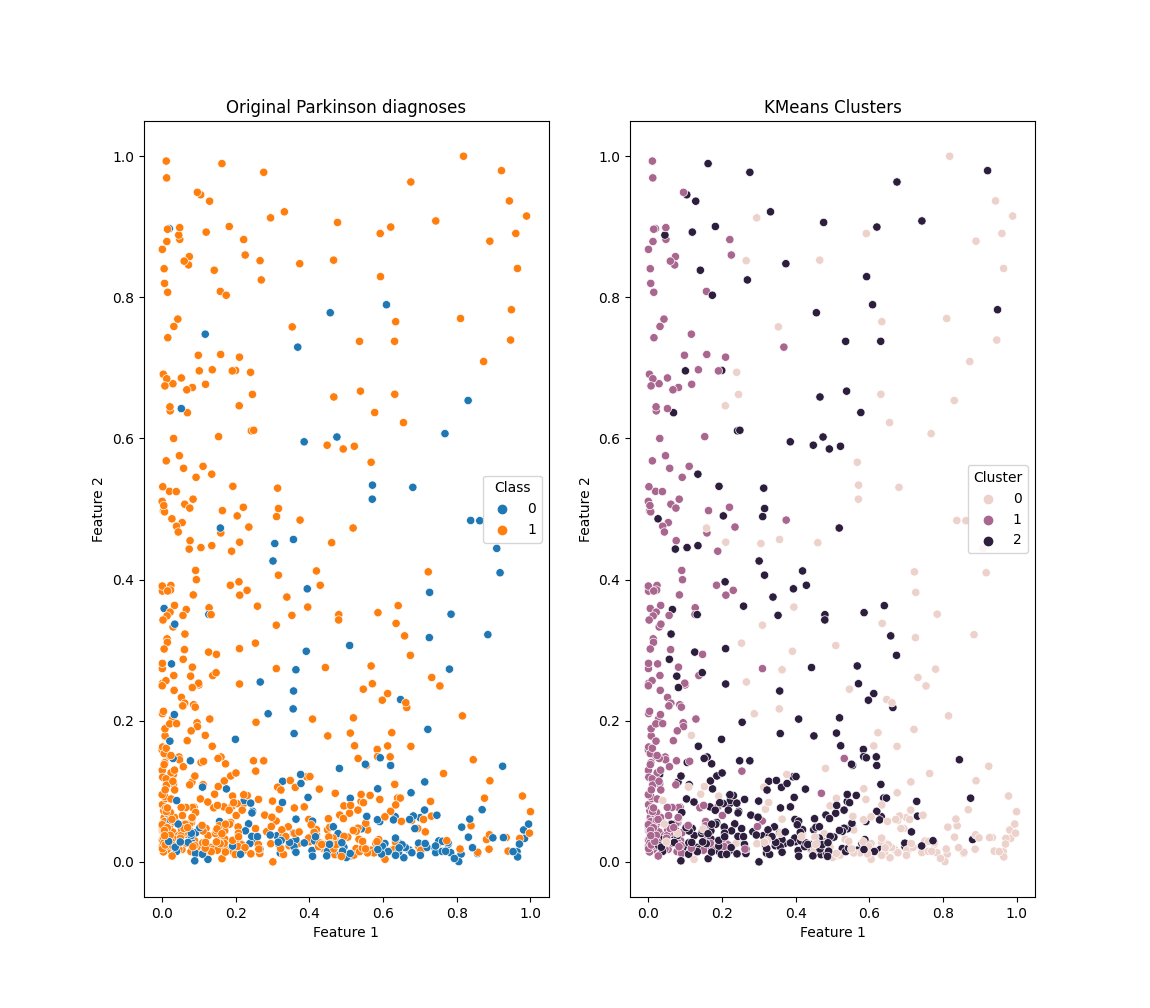
\includegraphics[width=\textwidth,valign=t]{scatter}
		      \caption{Scatter Plot}
	      \end{figure}

	\item The number of principal components required to explain more than 80\% of
	      the variance is 31.
\end{enumerate}
\pagebreak

\section{Appendix}
\lstinputlisting[language=Python]{./src/code.py}

\end{document}
